For the main control of the system, a State Machine with singleton pattern design is used. Every state is designed to be as small as possible. For the German Open 2015, we implemented three main states divided on smaller sub-states: move, grasp and deliver (see figure~\ref{fig:SM})\todo{jon: things mentioned here should stick with the image}.

Once we get the tasks from the referee box, the first step for every test is to drive to a specific position and an specific orientation. Once we are on the desired position we smoothly approach to the service area and perform the task of grasping or delivering an object. 	

\begin{figure}[htbp]
	\centering
	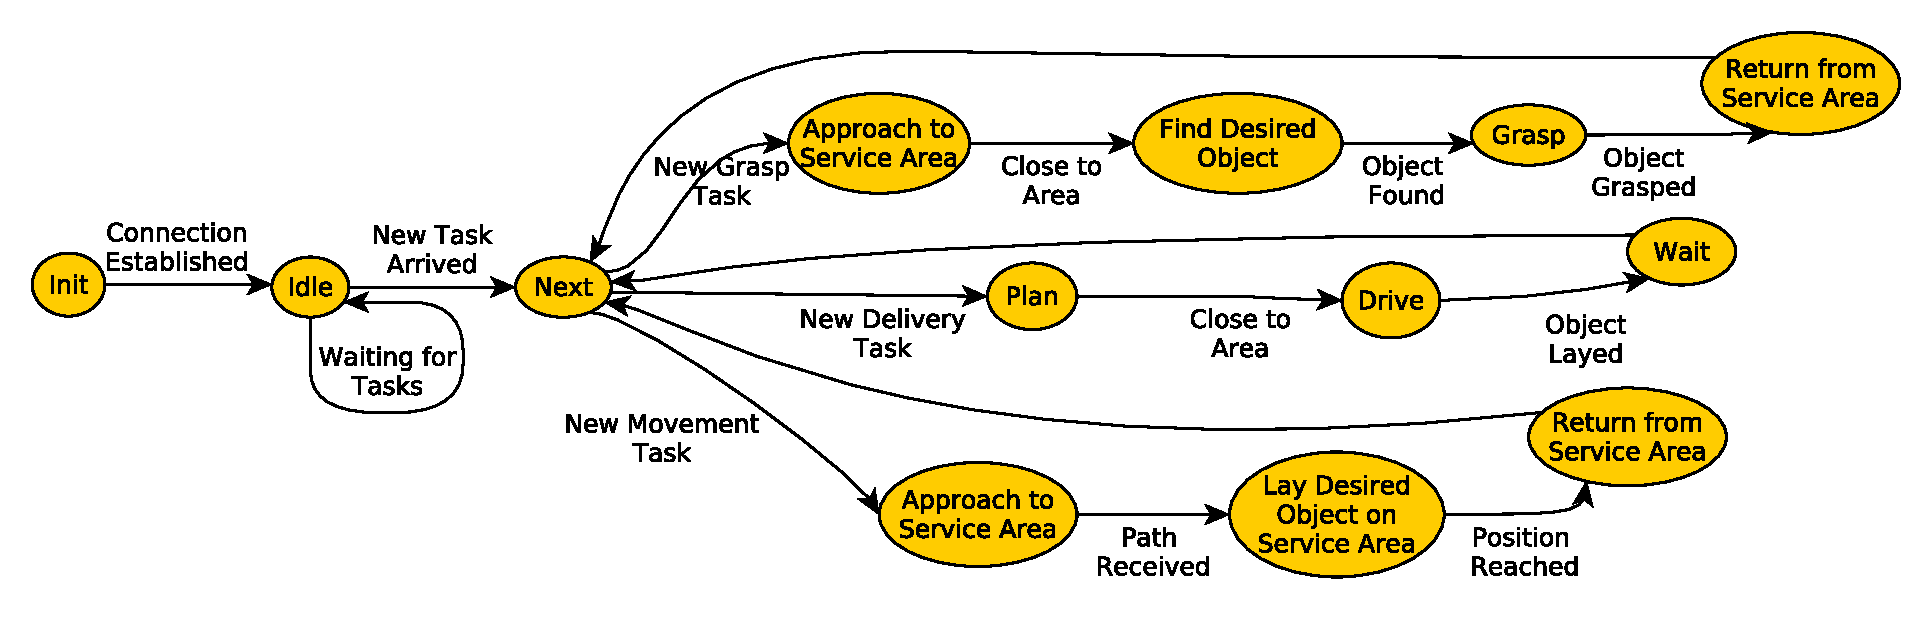
\includegraphics[width=\textwidth]{img/sm}
	\caption{Structure of the Statemachine}
	\label{fig:SM}
\end{figure}


The State Machine framework could be found on GitHub under our Laboratory's repository: "autonohm/obviously". 